% ----------------------------------------------------------------
% AMS-LaTeX Paper ************************************************
% **** -----------------------------------------------------------
\documentclass{amsart}
\usepackage{graphicx}
\usepackage{listings}
\usepackage{float}
\usepackage[table]{xcolor}
\usepackage[margin=1in]{geometry}
\usepackage[fontsize=12bp]{fontsize}
\graphicspath{ {./images/} }

% ----------------------------------------------------------------
\vfuzz2pt % Don't report over-full v-boxes if over-edge is small
\hfuzz2pt % Don't report over-full h-boxes if over-edge is small
\begin{document}

\title{COP5522\\{\bf Project Report}}%
\author{Dae Hyun Sung and Farooq Mahmud}%
\date{}

%\dedicatory{}%
%\commby{}%
% ----------------------------------------------------------------

\maketitle\

\section{Introduction}
In this project we demonstrate optimizations made on a recursive implementation of a Fast Fourier Transform (FFT). The FFT algorithm takes samplings of multiple sine waves for the period
$2\pi$ and sums the samples to create a complex waveform upon which to perform the FFT. We successfully recreated a recursive version of the well-known Cooley-Tukey algorithm whose main advantage is its $\Theta(n\log n)$ runtime as opposed to the $\Theta(n^{2})$ runtime of the straightforward implementation~\cite{cormen}. After benchmarking the recursive implementation we proceeded to benchamark an iterative version adapated from an open source implementation~\cite{rshuston}. The iterative version showed drasitaclly reduced runtimes. Lastly, we improved the runtime of the iterative implementation by parallelizing two  \textbf{for} loops using the OpenMP library. Subsequent sections cover the testing methodology and compare the execution times of three implementations based on the varying number of threads. Lastly the scalability and efficiency metrics of the parallelized iterative implementation are presented.

All experiments were performed on the Ubuntu 20.04 operating system equipped with an Intel I7 2.8GHz processor having four physical cores and eight logical cores. All programs were run with the \textbf{-O3} \textbf{gcc} compiler optimization flag.

The algorithm exepects input sizes that are powers of two. There are solutions involving non-powers of two, but those complicate the code without providing any additional insight into the performance~\cite{cormen}. In the parallel case, the number of threads must be powers of two. This assumption simplifies the code.

Appendix \ref{appendix:codefiles} lists the structure of the code files for the three implementations. Instructions for building the three executables are in Appendix \ref{appendix:building}. Instructions for running the three executables are in Appendix \ref{appendix:running}.

The video demonstration for this project can be viewed at https://youtu.be/iUrCV7SN1nw.


\section{Testing Methodology}
To ensure meaningful runtime values, the input sample size must be adequately large. For the tests, a sample size of $2^{22}$ samples is used. The tests generate three cosine waves. The first waveform has frequency of one and an amplitude of ten. The second waveform has frequency of two and an amplitude of four. The third waveform has frequency of four and an amplitude of five (Figure~\ref{figure:input-waveforms}). We generate the samples over a period of $2\pi$, and the summed waveform (Figure~\ref{figure:summed-waveform}) is used as the input for the FFT calculation. The FFT results are shown in Figure~\ref{figure:fft-result}

\begin{figure}[htbp]
\caption{Input waveforms.}
\begin{center}
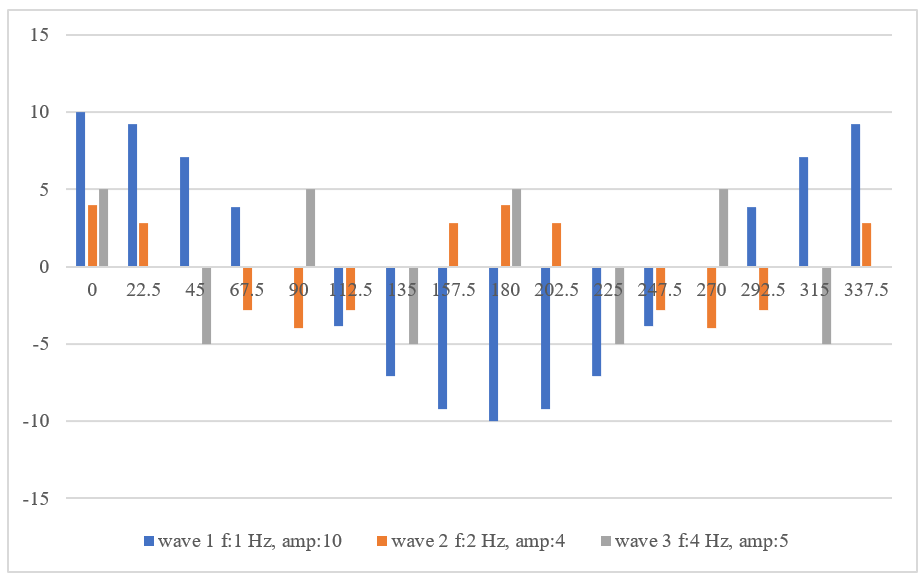
\includegraphics{input-waveforms.PNG}
\end{center}
\label{figure:input-waveforms}
\end{figure}

\begin{figure}[H]
\caption{Summed waveforms.}
\begin{center}
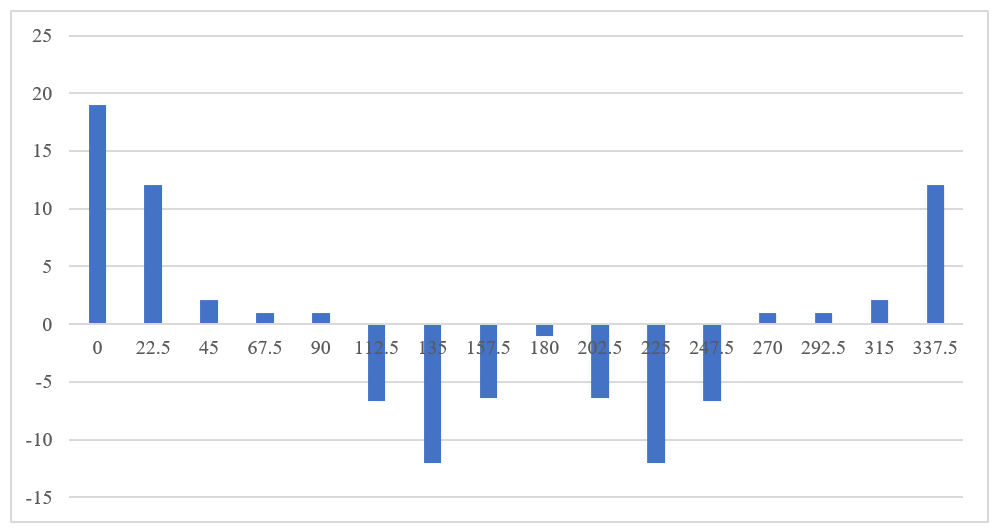
\includegraphics{summed-waveform.PNG}
\end{center}
\label{figure:summed-waveform}
\end{figure}

\begin{figure}[htbp]
\caption{FFT results.}
\begin{center}
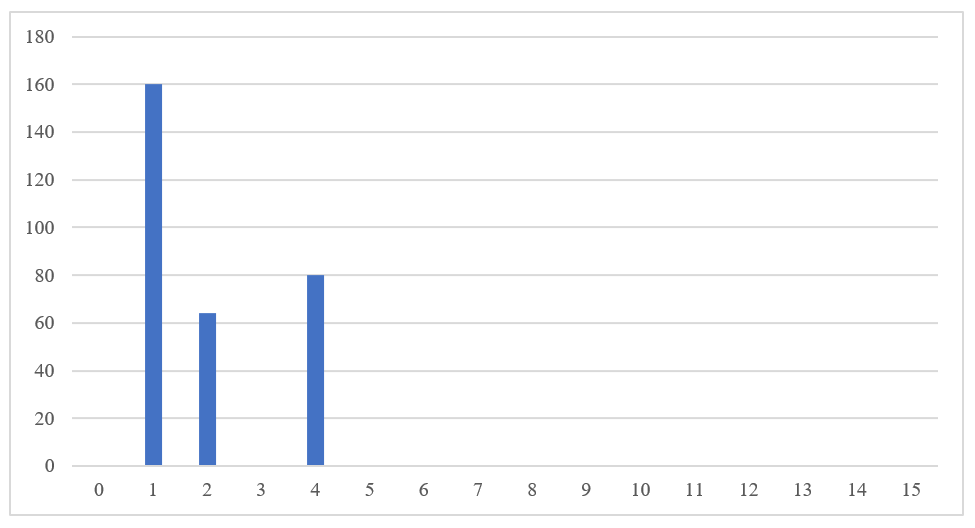
\includegraphics{fft-result.PNG}
\end{center}
\label{figure:fft-result}
\end{figure}

To test correctness, we perform the FFT and get the correct resulting FFT graph with the correct frequency values and relative amplitudes in the input waves. We will take the runtime average of ten runs, and use the average values to normalize runtime fluctuations. We use the same sample size to test the three implementations. We then compare the runtimes between all three implementations, and analyze the scalability and efficiency of the parallelized openMP algorithm.

\section{Comparison of Serial and Iterative Serial Runtimes}

Figure~\ref{figure:serial-vs-iterative-serial} shows the runtimes of the recursive and serial iterative implementations for an input size of $2^{22}$. Recursion generally performs worse than its iterative counterpart due to stack maintenance overhead~\cite{bryant}. The iterative version is faster because the calculations involve iterating over local variables, i.e. there is a less stack maintenance overhead.

\begin{figure}[htbp]
\caption{Serial runtime vs. iterative serial runtime.}
\begin{center}
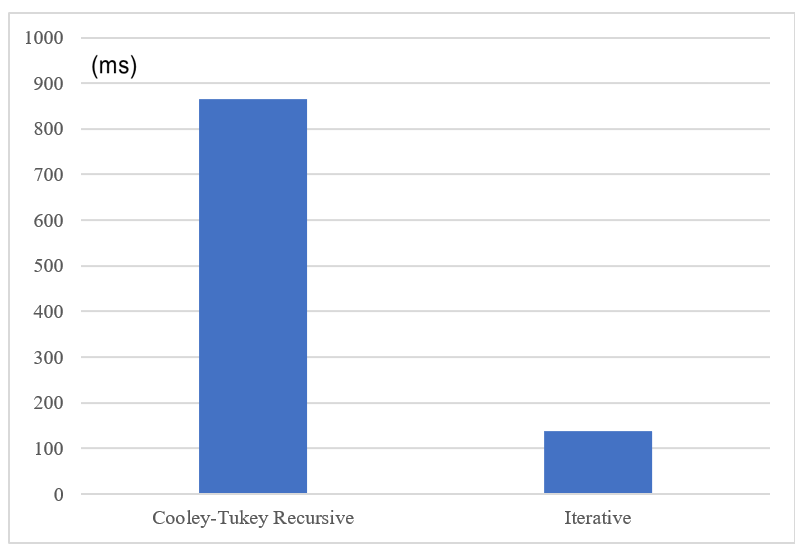
\includegraphics{serial-vs-iterative-serial.PNG}
\end{center}
\label{figure:serial-vs-iterative-serial}
\end{figure}


\section{Parallel Iterative Implementation}
The iterative algorithm was parallelized using the OpenMP library. Two \textbf{for} loops were parallelized. The code for these methods are on lines 50 - 124 in \textbf{fft.c}. Figure~\ref{figure:parallel} shows the runtimes for varying number of threads.

\begin{figure}[H]
\caption{Parallel runtimes.}
\begin{center}
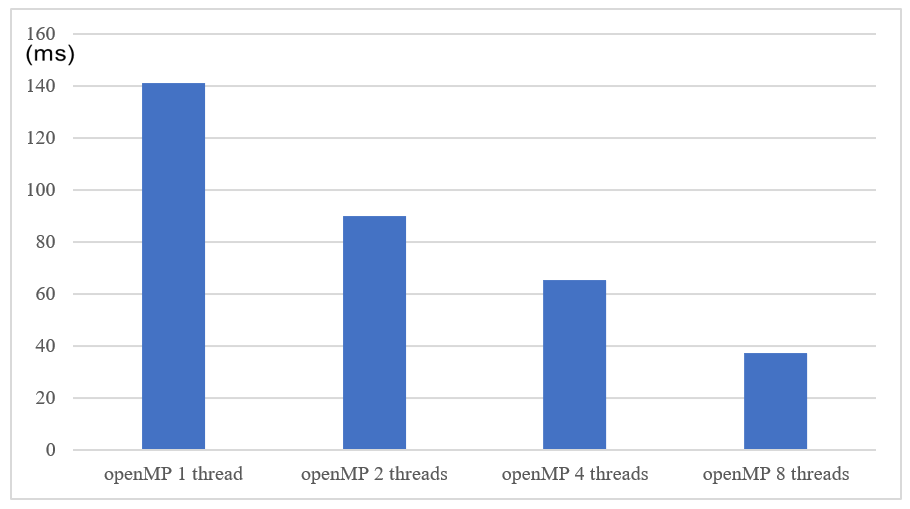
\includegraphics{parallel.PNG}
\end{center}
\label{figure:parallel}
\end{figure}



\subsection{Speedup and Efficiency}
Speedup and efficiency are two common metrics used for evaluating the performance of a parallel algorithm against the serial version~\cite{pacheco}. Speedup is the improvement in parallel execution time over the serial implementation, as shown in Equation~\ref{eq:speedup}.

\begin{equation}
Speedup = \frac{T_{serial}}{T_{parallel}}
\label{eq:speedup}
\end{equation}

Efficiency is the relative improvement in execution time as the number of processes increase, as shown in Equation~\ref{eq:efficiency}. 

\begin{equation}
Efficiency = \frac{Speedup}{number\,of\,processes}
\label{eq:efficiency}
\end{equation}

Table~\ref{table:speedup-efficency} reports the speedup and efficiency values for varying number of threads. Figures~\ref{figure:speedup} and ~\ref{figure:efficiency} depicts these values graphically. 

\begin{table}[htbp]
\caption{Speedup and Efficiency}
\begin{center}
\rowcolors{2}{gray!10}{gray!40}
\begin{tabular}{|c|c|c|}
\hline
Number of processes & Speedup & Efficiency \\
\hline
1 & 1.0 & 1.0   \\
2 & 1.57 & 0.78 \\
4 & 2.16 &  0.54 \\
8 & 3.77 & 0.47 \\
\hline
\end{tabular}
\end{center}
\label{table:speedup-efficency}
\end{table}

\begin{figure}[H]
\caption{Speedup}
\begin{center}
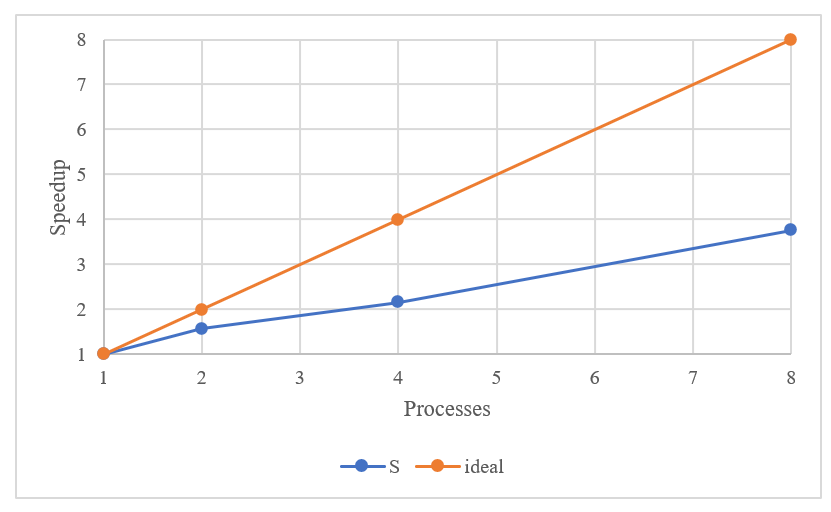
\includegraphics{speedup.PNG}
\end{center}
\label{figure:speedup}
\end{figure}

\begin{figure}[H]
\caption{Efficiency}
\begin{center}
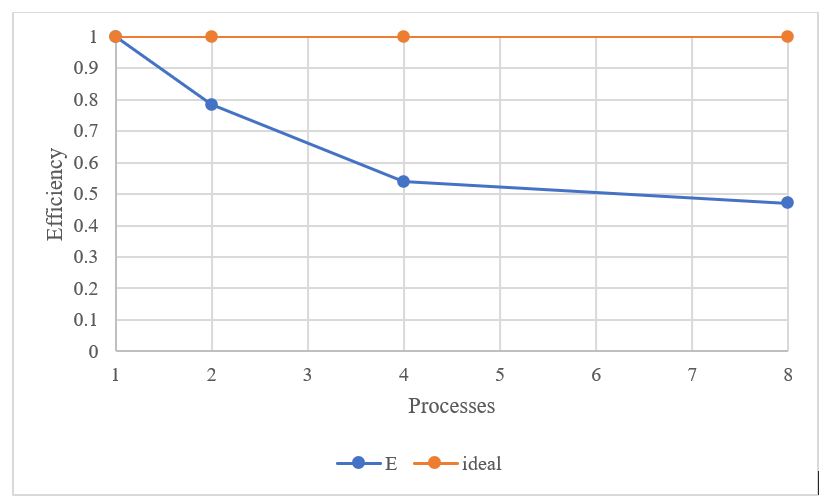
\includegraphics{efficiency.PNG}
\end{center}
\label{figure:efficiency}
\end{figure}

\section{Conclusion}
In this assignment, the serial recursive, serial iterative, and parallel implementations of the Cooley-Tukey Fast Fourier Transform algorithm were compared. Not surprisingly, the recursive version was the slowest. The serial iterative version was much faster due to less stack maintenance overhead. Parallelizing the iterative implementation improved the runtime even more as evidenced by the increased speedup metric. The key takeaways from the project are (1) prefer an iterative solution over a recursive one if performance is of prime importance and (2) consider parallelizing an iterative algorithm using OpenMP as a way to increase performance further without over-complicating the code.

\bibliographystyle{plain}
\bibliography{COP5520-project-report}

\pagebreak

\appendix

\section{Code Files}\label{appendix:codefiles}
The three implmentations are contained in three separate folders according to Table~\ref{table:codefiles}.

\begin{table}[H]
\caption{Code files}
\begin{center}
\rowcolors{2}{gray!10}{gray!40}
\begin{tabular}{|c|c|}
\hline
Implementation & Folder name \\
\hline
Serial & \text{fft\_serial} \\
Serial iterative & \text{fft\_iterative} \\
Parallel & \text{fft\_openMP}  \\
\hline
\end{tabular}
\end{center}
\label{table:codefiles}
\end{table}

\section{Building the Executables}\label{appendix:building}
Each implementation's folder contains a \text{makefile}. To build the executable for the serial implementation for example, run  \textbf{make clean} followed by \textbf{make} in the \text{fft\_serial} folder. The makefiles generate the following executables:

\begin{enumerate}
\item  \textbf{fft\_serial}/\textbf{fft\_serial.exe}
\item \textbf{fft\_iterative}/\textbf{fft\_iterative.exe}
\item \textbf{fft\_openMP}/\textbf{fft\_openMP.exe}
\end{enumerate}

\section{Running the Executables}\label{appendix:running}
Table~\ref{table:execution} shows the command lines used to run the programs. The first argument of each program is the number of samples as a power of two. For example, to run a program with 16 samples, the first argument is 4. The second argument to the parallel implementation is the number of threads which must be a power of two. If \textbf{-\phantom{}-print} is passed to any program as the last parameter, the input and output waveforms are printed to the console.

\begin{table}[htbp]
\caption{Command lines}
\begin{center}
\rowcolors{2}{gray!10}{gray!40}
\begin{tabular}{|p{0.2\textwidth}|p{0.5\textwidth}|}
\hline
Implementation & Command \\
\hline
Serial & \textbf{./fft\_serial [samples]} \\
Serial iterative & \textbf{./fft\_iterative [samples]} \\
Parallel & \textbf{./fft\_openMP [samples] [threads]} \\
\hline
\end{tabular}
\end{center}
\label{table:execution}
\end{table}

\end{document}
